% YOLO Final 项目代码速览与汇报辅助总结。
% 本 PDF 不是正式实验论文，而是现场看代码讲项目时的辅助材料。
\documentclass[11pt,a4paper]{article}

\usepackage{fontspec}
\setmainfont{Noto Serif CJK SC}
\setsansfont{Noto Sans}
\setmonofont{Noto Sans Mono}
\usepackage[a4paper,margin=0.85in]{geometry}
\usepackage{graphicx}
\usepackage{booktabs}
\usepackage{longtable}
\usepackage{float}
\usepackage{hyperref}
\usepackage{array}
\usepackage{amsmath}
\usepackage{amssymb}
\usepackage{enumitem}
\usepackage{xcolor}
\usepackage{fancyvrb}

\setlength{\parskip}{0.45em}
\setlength{\parindent}{2em}
\renewcommand{\arraystretch}{1.18}

\newcommand{\code}[1]{\texttt{#1}}
\newcommand{\file}[1]{\path{#1}}

\title{YOLO Final 项目代码速览与汇报辅助总结}
\author{}
\date{2026-05-15}

\begin{document}

\maketitle
\tableofcontents
\newpage

\section{这份 PDF 的用途}

这份 PDF 的目的不是替代正式报告，而是帮助现场汇报时按代码讲清楚项目。现场如果只能打开代码，建议按照下面顺序讲：

\begin{enumerate}[label=\arabic*.]
  \item 先讲 \code{configs/}：最终实验到底怎么配置；
  \item 再讲 \code{models/}：backbone、neck、head 如何组成检测器；
  \item 再讲 \code{data/}：COCO-only、\code{.pt} packed loader 和 bbox 处理；
  \item 再讲 \code{losses/}：动态分配、GIoU、objectness、classification loss；
  \item 再讲 \code{tools/train\_ddp.py} 与 \code{engine/distributed\_trainer.py}：8GPU DDP 如何训练；
  \item 再讲 \code{utils/coco\_eval.py}：为什么我们的指标可信；
  \item 最后讲 \code{tools/export\_model.py}、\code{tools/quantize\_model.py} 和前后端：模型如何部署。
\end{enumerate}

\section{项目最终成果}

最终我们完成的是一个可训练、可评估、可对比、可导出、可量化、可部署的 YOLO 目标检测系统。最终主线模型为：

\begin{itemize}
  \item 模型：\code{deep\_residual\_dual\_scale\_three\_box}
  \item 输入尺寸：416 $\times$ 416
  \item 检测尺度：p4 / p5 双尺度
  \item 每尺度 anchors：3 个
  \item 类别数：COCO 80 类
  \item 数据读取：COCO-only \code{.pt} packed loader
  \item 训练：8GPU DDP，50 epoch，AdamW + cosine scheduler，学习率 $7\times10^{-4}$
  \item 增广：train-only bbox-safe basic augmentation + scale jitter
  \item 部署：TorchScript 导出，backbone INT8 + head FP32 量化版本
\end{itemize}

最终最佳 FP32 checkpoint：

\begin{Verbatim}[fontsize=\small]
yolo_final/outputs/
dual_scale_three_box_coco_only_noobj1_416_basic_aug_scale_jitter_50_lr7e4_ddp_20260512_130823/best.pth
\end{Verbatim}

完整 COCO val2017 指标如下：

\begin{table}[H]
\centering
\begin{tabular}{lr}
\toprule
指标 & 数值 \\
\midrule
COCO AP & 0.192170 \\
AP50 & 0.310452 \\
AP75 & 0.200965 \\
AP small & 0.084709 \\
AP medium & 0.211648 \\
AP large & 0.261832 \\
AR100 & 0.351947 \\
\bottomrule
\end{tabular}
\end{table}

\section{代码目录应当怎么讲}

\begin{longtable}{p{0.24\textwidth}p{0.68\textwidth}}
\toprule
目录或文件 & 现场讲解重点 \\
\midrule
\file{configs/} & 所有正式实验都由 TOML 配置驱动。最终配置为 \file{dual_scale_three_box_coco_only_noobj1_416_basic_aug_scale_jitter_50_lr7e4.toml}。\\
\file{models/common.py} & 基础模块：\code{ConvBNAct}、\code{ResidualBlock}、\code{BasicResidualBlock}。\\
\file{models/backbone.py} & 多尺度 backbone：逐级下采样，输出 p4/p5，必要时输出 p3。\\
\file{models/neck.py} & \code{DualScaleFPNPANLite}，负责 FPN/PAN-lite 多尺度特征融合。\\
\file{models/head.py} & \code{DecoupledDetectionHead}，分类分支和回归/objectness 分支解耦。\\
\file{models/detector.py} & \code{YOLOv0Baseline}，统一组装 backbone、neck、head。\\
\file{data/detection_dataset.py} & COCO manifest 读取、\code{.pt} packed loader、resize、bbox sanitize、collate。\\
\file{losses/yolo_loss.py} & GIoU、objectness、classification loss、dynamic cost assignment。\\
\file{engine/distributed_trainer.py} & DDP 下每个 epoch 的训练、验证、全局指标聚合。\\
\file{tools/train_ddp.py} & 8GPU DDP 正式训练入口。\\
\file{utils/prediction.py} & prediction tensor 解码、score 计算、NMS。\\
\file{utils/coco_eval.py} & pycocotools 正式 COCO AP 评估，含原图坐标映射。\\
\file{tools/sweep_coco_checkpoint.py} & 非训练 sweep，选择 score/NMS/top-k 展示参数。\\
\file{tools/export_model.py} & TorchScript/ONNX 导出入口。\\
\file{tools/quantize_model.py} & INT8 量化和 calibration。\\
\file{backend/}、\file{frontend/} & 可直接上传图片使用的 YOLO 检测工具。\\
\bottomrule
\end{longtable}

\section{最终网络结构}

\subsection{整体检测器}

总入口在 \file{models/detector.py}。核心思想是把模型拆成三段：

\[
\text{image} \rightarrow \text{backbone features} \rightarrow \text{neck fused features} \rightarrow \text{prediction tensors}
\]

代码中对应：

\begin{Verbatim}[fontsize=\small]
features = self.backbone(x)
if self.neck is not None:
    features = self.neck(features)
return {level: self.head[level](features[level]) for level in self.feature_levels}
\end{Verbatim}

最终配置下：

\begin{itemize}
  \item backbone 输出 p4、p5；
  \item neck 对 p4、p5 做 FPN/PAN-lite 融合；
  \item head 在 p4、p5 上分别输出检测 tensor；
  \item 每个尺度每个 grid 预测 3 个 anchors；
  \item 每个 anchor 输出 4 个 box 参数、1 个 objectness、80 个类别 logits。
\end{itemize}

\subsection{Backbone 理论设计}

backbone 的作用是从图像中提取层级特征。浅层特征保留边缘、纹理和局部结构；深层特征分辨率更低，但语义更强。

最终使用 \code{MultiScaleBaselineBackbone}。其结构是多个 stage 串联，每个 stage 由若干 \code{ConvBNAct} 和可选 \code{ResidualBlock} 组成，并通过 pooling 逐步下采样。

核心模块为：

\begin{Verbatim}[fontsize=\small]
class ConvBNAct:
    Conv2d -> BatchNorm2d -> ReLU

class ResidualBlock:
    y = x + ConvBNAct(ConvBNAct(x))
\end{Verbatim}

残差连接的理论意义是让深层网络学习残差映射：

\[
y = x + F(x)
\]

相比直接学习 $y=F(x)$，残差结构更容易优化，可以缓解深层网络训练中的梯度传播问题。

最终 backbone 输出：

\begin{itemize}
  \item p4：更高空间分辨率，适合中小目标；
  \item p5：更强语义表达，适合中大目标。
\end{itemize}

\subsection{Neck 理论设计}

neck 使用 \code{DualScaleFPNPANLite}。它的目标是融合不同层级特征，让每个检测尺度同时拥有语义信息和定位信息。

FPN top-down 路径：

\[
P4_{td} = \text{Conv}_{3\times3}\left(\text{Conv}_{1\times1}(P4) + \text{Upsample}(\text{Conv}_{1\times1}(P5))\right)
\]

PAN bottom-up 路径：

\[
P5_{out} = \text{Conv}_{3\times3}\left(\text{Conv}_{1\times1}(P5) + \text{Downsample}(P4_{out})\right)
\]

代码中的关键操作：

\begin{Verbatim}[fontsize=\small]
p5_td = self.p5_lateral(p5)
p5_up = F.interpolate(p5_td, size=p4.shape[-2:], mode="nearest")
p4_td = self.p4_fuse(self.p4_reduce(p4) + p5_up)

p4_down = self.p4_downsample(p4_out)
p5_out = self.p5_fuse(self.p5_reduce(p5) + p4_down)
\end{Verbatim}

理论上，FPN 把高层语义传给高分辨率特征，PAN 把低层定位信息再向上传递。这样 p4 和 p5 都不再是单一来源的 backbone 特征，而是融合后的检测特征。

\subsection{Head 理论设计}

最终使用 \code{DecoupledDetectionHead}。它把分类任务和回归/objectness 任务分开：

\begin{Verbatim}[fontsize=\small]
x = self.stem(x)
cls_feat = self.cls_branch(x)
reg_feat = self.reg_branch(x)

cls_logits = self.cls_pred(cls_feat)
reg_logits = self.reg_pred(reg_feat)
\end{Verbatim}

理论原因是分类和定位关注的信息不同：

\begin{itemize}
  \item 分类更依赖语义和类别判别；
  \item bbox 回归更依赖边界、中心点和尺度；
  \item objectness 更像候选框质量判断。
\end{itemize}

解耦 head 可以减少任务之间的梯度冲突。最终输出形状为：

\[
[B, H, W, A(5+C)]
\]

其中 $A=3$，$C=80$，所以每个尺度的最后一维是：

\[
3\times(5+80)=255
\]

\section{Prediction Tensor 到 Detection Result}

模型输出的是 prediction tensor，不是最终框。最终检测结果需要经过四步：

\begin{enumerate}[label=\arabic*.]
  \item 按 YOLOv5 风格参数化解码 bbox；
  \item 对 objectness 和 class logits 做 sigmoid；
  \item 计算最终分数；
  \item NMS 去重并保留 top-k。
\end{enumerate}

最终分数为：

\[
\text{score} = \text{objectness}^{\alpha} \cdot \text{class\_score}^{\beta}
\]

最终主线评估和展示常用：

\[
\alpha=2.0,\quad \beta=1.0
\]

这表示我们更强调 objectness 的质量校准。

\section{Loss 与正样本分配}

最终 loss 由四部分构成：

\[
L =
\lambda_{box} L_{box}
+ \lambda_{obj} L_{obj}^{pos}
+ \lambda_{noobj} L_{obj}^{neg}
+ \lambda_{cls} L_{cls}
\]

最终配置为：

\begin{table}[H]
\centering
\begin{tabular}{ll}
\toprule
参数 & 含义 \\
\midrule
\code{lambda\_box=5.0} & 提高定位损失权重，因为 COCO AP 对定位质量敏感。\\
\code{lambda\_obj=1.0} & 正样本 objectness 权重。\\
\code{lambda\_noobj=1.0} & 背景 objectness 权重，用于抑制误检。\\
\code{lambda\_cls=1.0} & 分类损失权重。\\
\code{dynamic\_topk=2} & 每个 GT 最多选择 2 个低 cost 正样本。\\
\code{soft\_objectness\_target=iou} & 用 IoU 作为 objectness soft target。\\
\code{cls\_loss\_mode=quality\_bce} & BCE 形式，类别 target 可由 IoU soft target 调整。\\
\bottomrule
\end{tabular}
\end{table}

正样本分配采用 \code{dynamic\_cost}。它不是固定把 GT 分给某一个 anchor，而是在候选中心区域中按定位 cost 和分类 cost 选择候选：

\[
cost = 3.0\cdot cost_{box} + 1.0\cdot cost_{cls}
\]

这个设计的核心意义是让训练中真正负责某个 GT 的候选更接近当前模型的预测质量。

\section{数据读取与数据增广}

\subsection{COCO-only 数据口径}

最终训练和评估都使用 COCO-only：

\begin{Verbatim}[fontsize=\small]
train_manifest = /home/lidz/YOLO/DataSet/Unified/manifests/coco2017_train.jsonl
val_manifest   = /home/lidz/YOLO/DataSet/Unified/manifests/coco2017_val.jsonl
num_classes    = 80
\end{Verbatim}

我们不再直接混合 VOC 和 COCO，因为二者 label id 语义不同。COCO-only 保证类别空间、训练标签和 COCO AP 评估一致。

\subsection{.pt packed loader}

最终使用 \code{.pt} packed chunks 读取数据：

\begin{Verbatim}[fontsize=\small]
packing_format = "pt"
packed_root = "/home/lidz/YOLO/DataSet/Unified/packed"
packed_chunk_size = 1024
packed_cache_size = 4
\end{Verbatim}

作用是降低大量小文件随机 IO，提高 8GPU DDP 训练时的数据供给稳定性。启动时会调用 \code{validate\_packed\_index}，提前检查 index、chunk、格式和样本数量。

\subsection{保守数据增广}

最终增广策略是 train-only 且 bbox-safe：

\begin{itemize}
  \item horizontal flip；
  \item color jitter；
  \item light scale jitter；
  \item light affine；
  \item bbox sanitize。
\end{itemize}

增广后必须同步更新 bbox，并裁剪或删除无效框。检测任务中如果图片变换和 bbox 没有同步，训练标签会直接错误。

\section{训练链路}

正式训练入口是 \file{tools/train\_ddp.py}。启动方式：

\begin{Verbatim}[fontsize=\small]
torchrun --standalone --nproc_per_node=8 \
  tools/train_ddp.py \
  --config configs/dual_scale_three_box_coco_only_noobj1_416_basic_aug_scale_jitter_50_lr7e4.toml
\end{Verbatim}

DDP 训练流程：

\begin{enumerate}[label=\arabic*.]
  \item rank0 初始化实验目录，生成 \code{run\_id}、config snapshot、metadata；
  \item 所有 rank 读取同一配置；
  \item 每个 rank 绑定一个 GPU；
  \item 使用 \code{DistributedSampler} 划分数据；
  \item 使用 \code{DistributedDataParallel} 包装模型；
  \item rank0 写 TensorBoard 和 checkpoint；
  \item 每个 epoch 汇总全局 loss、sample count、optimizer steps。
\end{enumerate}

我们专门修正了 DDP 日志语义：

\begin{itemize}
  \item \code{optimizer\_steps}：真正的 optimizer step 数；
  \item \code{global\_batch\_count}：所有 rank local batch 总数；
  \item \code{sample\_count}：全局样本数；
  \item epoch loss 按 sample count 加权平均。
\end{itemize}

\section{正式评估与可视化}

正式指标使用 \code{utils/coco\_eval.py} 和 pycocotools，而不是只看简化 mAP@0.5。

COCO AP 评估前必须把预测框从 resize 坐标映射回原图坐标：

\begin{Verbatim}[fontsize=\small]
original_height, original_width = target["original_size"].tolist()
scale_x = original_width / image_size
scale_y = original_height / image_size

x1 = x1 * scale_x
y1 = y1 * scale_y
x2 = x2 * scale_x
y2 = y2 * scale_y
\end{Verbatim}

否则 COCO GT 和预测框不在同一个坐标空间，AP 会接近 0。

每次正式实验结束后固定流程：

\begin{enumerate}[label=\arabic*.]
  \item full COCO val 评估；
  \item 500 图离线 sweep；
  \item 固定参数生成 12 张 pred-only 展示图；
  \item TensorBoard loss 曲线归档；
  \item metadata 和结果写入 \code{logs/records/}。
\end{enumerate}

\section{主要实验路线和结论}

\begin{longtable}{p{0.36\textwidth}rrrrp{0.22\textwidth}}
\toprule
实验 & AP & AP50 & AP75 & AR100 & 结论 \\
\midrule
320 COCO-only topk2 & 0.126985 & 0.218369 & 0.129184 & 0.260567 & COCO-only 起点。\\
320 topk1 & 0.108180 & 0.195980 & 0.105638 & 0.239071 & topk 降低伤害召回。\\
416 original & 0.148786 & 0.248717 & 0.155263 & 0.302299 & 分辨率提升明确有效。\\
416 K6 & 0.146778 & 0.244778 & 0.153023 & 0.303445 & 召回略好，AP 未超过原 anchors。\\
416 P3/P4/P5 K9 & 0.136481 & 0.228555 & 0.143862 & 0.313965 & AR 提升但 AP 下降。\\
416 scale jitter 40 & 0.181671 & 0.295159 & 0.189616 & 0.343730 & 数据增广主线有效。\\
416 scale jitter 50 lr1e-3 & 0.188057 & 0.307415 & 0.195546 & 0.348692 & 50 epoch 继续提升。\\
416 scale jitter 50 lr7e-4 & 0.192170 & 0.310452 & 0.200965 & 0.351947 & 最终最佳 FP32。\\
416 scale jitter 50 lr5e-4 & 0.190307 & 0.305895 & 0.200180 & 0.350863 & 接近但不如 7e-4。\\
\bottomrule
\end{longtable}

最终选择可以概括为：

\begin{Verbatim}[fontsize=\small]
COCO-only + 416 + p4/p5 + original anchors
+ residual backbone + FPN/PAN-lite neck + decoupled head
+ dynamic_topk=2 + lambda_noobj=1.0
+ bbox-safe augmentation + scale jitter
+ 50 epochs + AdamW/cosine + lr=7e-4 + 8GPU DDP
\end{Verbatim}

\section{我们犯过的关键错误}

这些错误是项目中最值得汇报的工程经验：

\begin{longtable}{p{0.28\textwidth}p{0.32\textwidth}p{0.32\textwidth}}
\toprule
错误 & 原因 & 修复 \\
\midrule
COCO AP 接近 0 & 预测框是 resize 坐标，GT 是原图坐标。 & 在 \code{utils/coco\_eval.py} 中映射回原图坐标。\\
VOC/COCO 混合训练 & VOC 和 COCO label id 语义不同。 & 正式实验改为 COCO-only。\\
\code{.pt} loader 未真正落地 & 配置写了 packed，但读取仍可能走 raw image。 & 补齐 \code{PackedPtStore} 和启动校验。\\
\code{positive\_cells} 统计错 & 多 anchor 下只统计 H/W，平均掉 anchor 维。 & 展平 \code{[H,W,A]} 后按图求和。\\
\code{quality\_bce} 语义不清 & 旧代码没有显式分支。 & 明确支持 \code{bce/quality\_bce/varifocal}。\\
训练过慢 & 早期使用 \code{DataParallel}。 & 改为 \code{torchrun} + 8GPU DDP。\\
DDP step 日志误导 & 把所有 rank batch 总数当 optimizer steps。 & 区分 \code{optimizer\_steps} 和 \code{global\_batch\_count}。\\
只看 val loss 误判 P3 & scale-aware 降低 loss，但 COCO AP 下降。 & 正式结论以 COCO AP/AR 和 sweep 为准。\\
可视化框数量不可比 & 4 张图和 12 张图使用不同阈值/top-k。 & 固定展示参数。\\
\bottomrule
\end{longtable}

\section{量化与部署}

\subsection{量化策略}

最终量化策略为：

\[
\text{Backbone INT8} + \text{Detection Head FP32}
\]

原因是 backbone 占主要卷积计算量，适合量化；head 直接输出 bbox、objectness 和 class logits，对数值更敏感。保留 head FP32 可以减少框偏移和分数排序损失。

量化 calibration 使用 COCO val manifest 前 128 张图片：

\begin{Verbatim}[fontsize=\small]
manifest = /home/lidz/YOLO/DataSet/Unified/manifests/coco2017_val.jsonl
calibration_samples = 128
input_size = 416 x 416
\end{Verbatim}

量化前后完整 COCO val 指标：

\begin{table}[H]
\centering
\begin{tabular}{lrrrr}
\toprule
模型 & AP & AP50 & AP75 & AR100 \\
\midrule
FP32 & 0.192170 & 0.310452 & 0.200965 & 0.351947 \\
INT8 backbone & 0.191483 & 0.309759 & 0.199871 & 0.351494 \\
\bottomrule
\end{tabular}
\end{table}

AP 只下降约 0.000687，说明 backbone-only INT8 是稳定的部署方案。

\subsection{量化样本展示}

量化校准样本的 HTML 图片墙和清单位于：

\begin{Verbatim}[fontsize=\small]
yolo_final/outputs/export_benchmark/checkpoint8_calibration128_samples/
  calibration128_gallery.html
  calibration128_samples.md
  calibration128_contact_sheet_all.jpg
\end{Verbatim}

\begin{figure}[H]
\centering
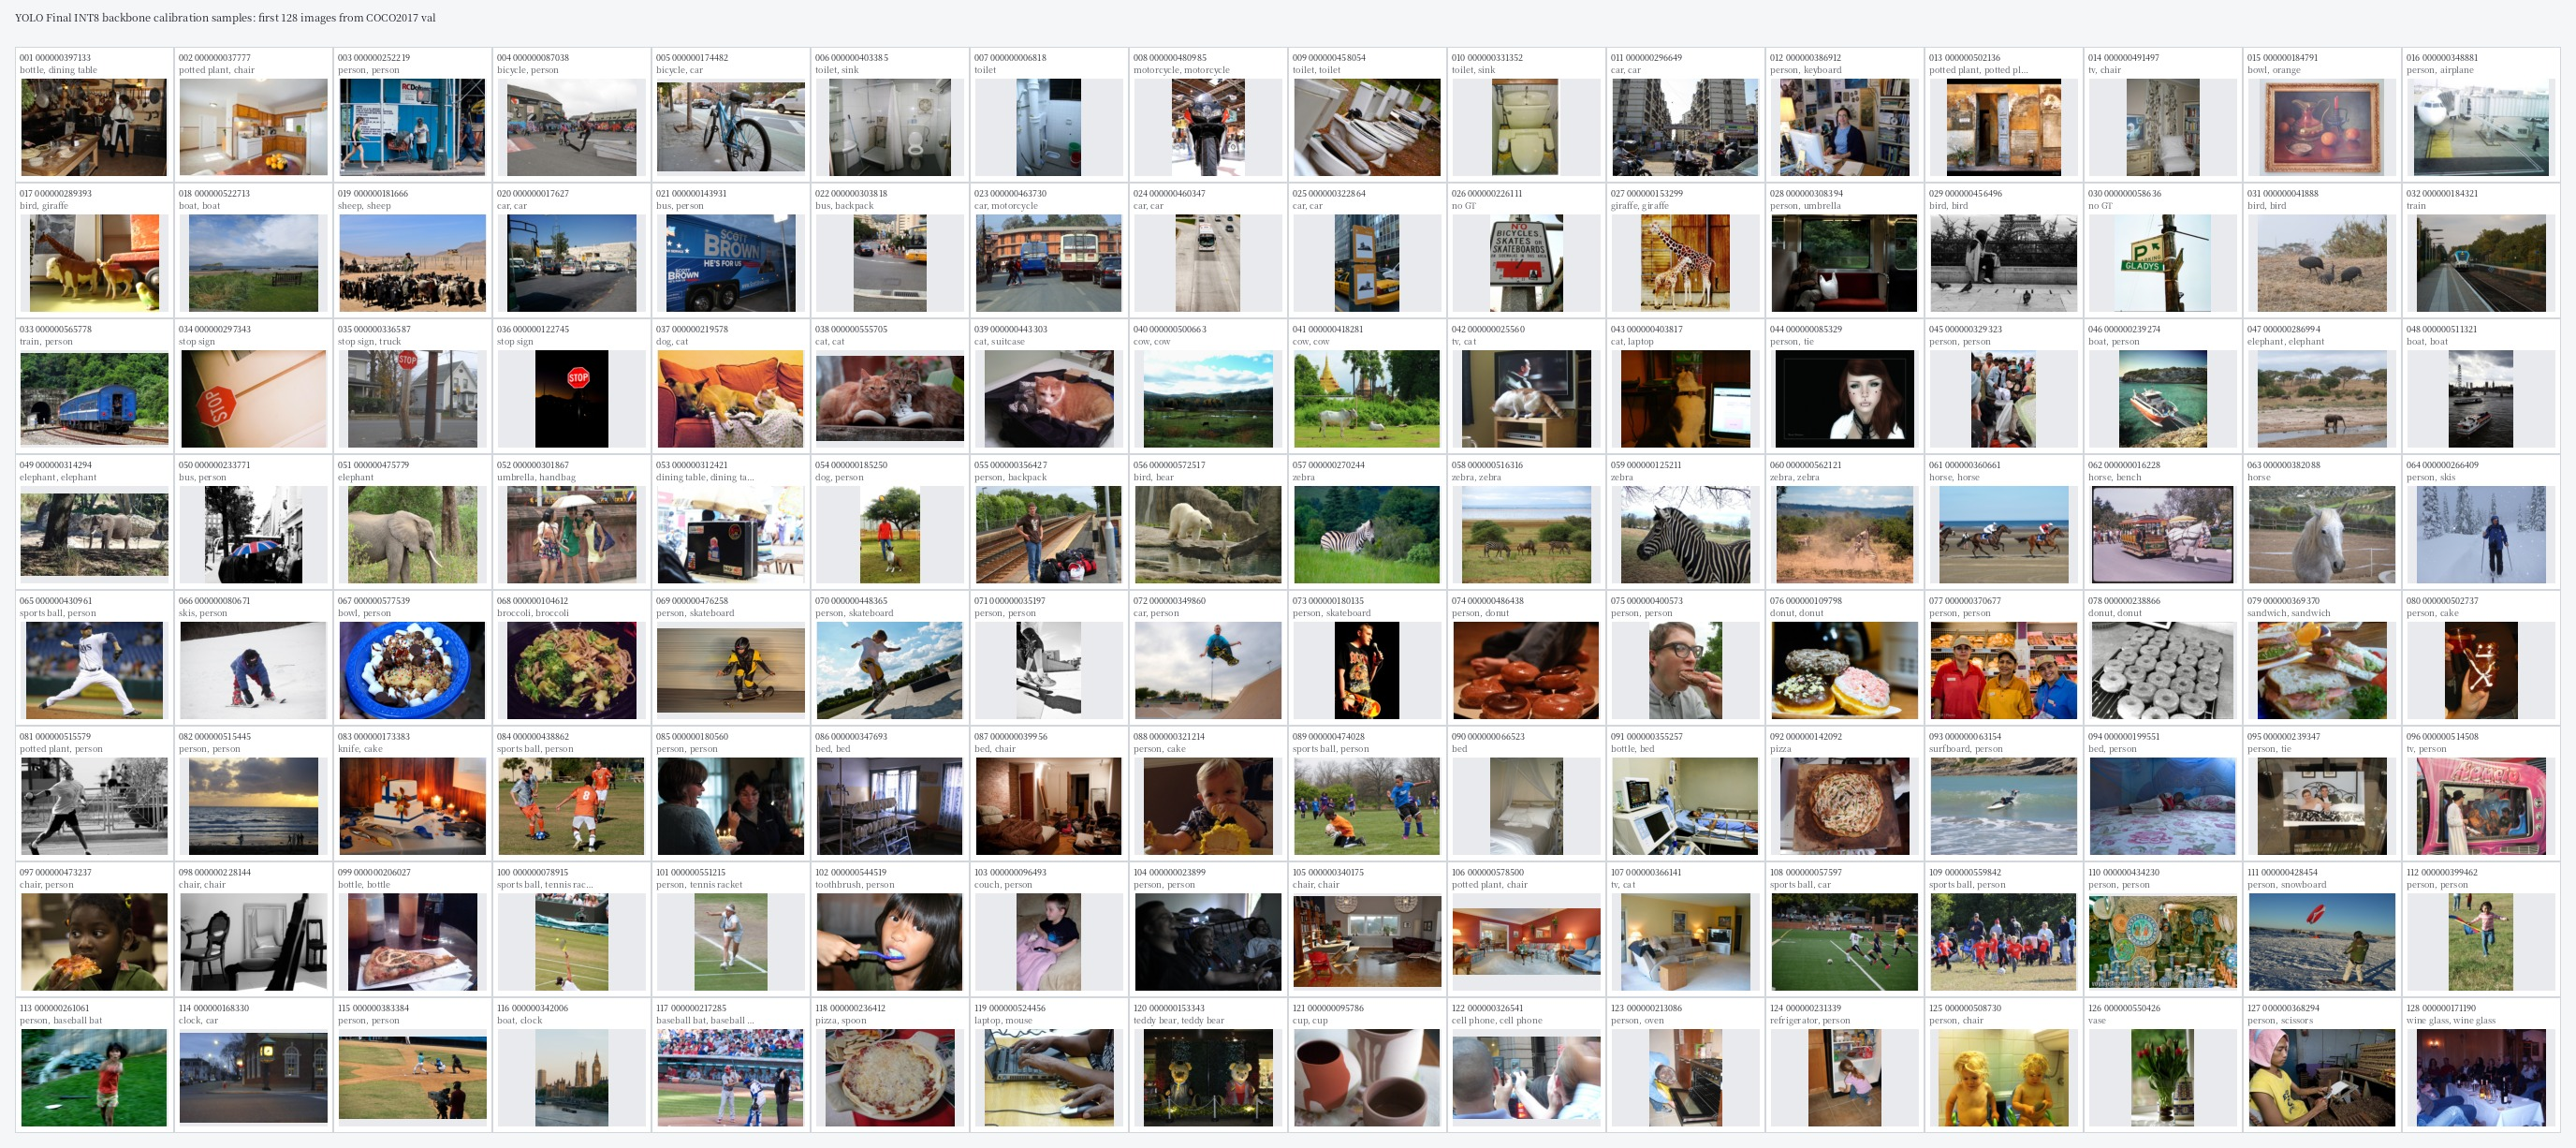
\includegraphics[width=\textwidth]{../outputs/export_benchmark/checkpoint8_calibration128_samples/calibration128_contact_sheet_all.jpg}
\caption{INT8 backbone calibration 使用的 128 张 COCO val 样本总览。}
\end{figure}

\subsection{前后端检测工具}

最终项目还包含可直接使用的检测工具：

\begin{Verbatim}[fontsize=\small]
scripts/start_yolo_detection_tool.sh
backend/
frontend/
\end{Verbatim}

后端加载导出的 TorchScript 模型，前端上传图片并展示检测框、类别、置信度和推理耗时。默认可使用 INT8 CPU 模型，也可以切换 FP32 GPU 模型。

\section{现场讲代码的建议路线}

如果现场只能打开代码，建议按下面顺序讲，每一步都能对应到具体文件：

\begin{enumerate}[label=\arabic*.]
  \item 打开最终配置文件，说明我们最终训练设置；
  \item 打开 \file{models/detector.py}，说明模型由 backbone、neck、head 组装；
  \item 打开 \file{models/backbone.py}，说明残差 stage 和 p4/p5 输出；
  \item 打开 \file{models/neck.py}，说明 FPN top-down 和 PAN bottom-up；
  \item 打开 \file{models/head.py}，说明 decoupled head 和输出 shape；
  \item 打开 \file{data/detection_dataset.py}，说明 COCO-only、packed loader、bbox sanitize；
  \item 打开 \file{losses/yolo_loss.py}，说明 dynamic assignment 和四个 loss term；
  \item 打开 \file{tools/train_ddp.py}，说明 8GPU DDP 如何启动；
  \item 打开 \file{utils/coco_eval.py}，说明评估坐标修复和 COCO AP；
  \item 打开 \file{tools/quantize_model.py}，说明 backbone INT8 + head FP32；
  \item 打开 \file{backend/} 和 \file{frontend/}，说明最终检测工具。
\end{enumerate}

\section{一句话总结}

这个项目最终完成了从 YOLO 检测模型设计、COCO-only 数据训练、8GPU DDP、正式 COCO AP 评估、实验消融、错误诊断、TorchScript 导出、INT8 量化到前后端检测工具的完整闭环。最重要的成果不是单一 AP 数字，而是建立了一条可信、可复现、可解释、可部署的目标检测工程链路。

\end{document}
